\documentclass[11pt]{article}
\usepackage{array}
\usepackage{tabularx}
\usepackage{graphicx}
\usepackage{algorithm}
\usepackage{algorithmic}
\usepackage{pgfplotstable}
\usepackage{pgfplots}
\usepackage{filecontents}
\usepackage{amsmath}

\title{
	\textbf{IMS Final Project Report}
}

\author{Tobias Stahl \\ 10528199 \and Ioannis-Giounous Aivalis \\ 10524851 }

\begin{document}

\maketitle

\section{Introduction}
In this report we will present the process followed in order to create an end-to-end system for image classification. The product system will perform image classification on four classes of images (airplanes, motorbikes, faces and cars) using the bag-of-words approach.
%TODO - alternative to the next sentense ?
The report is layed out as follows, first we will explain the theoretical aspect of how our model works. Then we will get more into technical details about how our system can be divided into logical units.

\section{Bag-of-Words based Image Classification}
In this section we will shortly describe the method used in order to achieve the final system. For classification we used the Bag-of-words approach. The rest of this section is divided into logical parts explaining the pipeline of the system as it was implemented and the series of actions it takes to get from plain input images to calssified output images.

The Bag-of-words approach originates from the Natural Language Processing and Information Retrieval fields. According to this method the document is represented by a bag (multiset) of words consisting it. These bags are later used for training a classifier on those documents.

Similarly, in the image case, each image is represented as a bag of words, the words being-this time, the descriptors the image consists of. More specifically, each of the images descriptors is assigned a word from a predefined vocabulary. All of these terms will be explained in the remaining of this section. 

\subsection{Feature Extraction and Description}
Each given image must undergo a preprocessing phase in order to be classified. In that directio, for each image that is processed by the system, a \emph{SiftImage} object is created. These objects now contain all the necessary information that might be required in future steps of the pipeline. More specifically, in the constructor of this class we extract various descriptors from which we will later have to decide which to use for training the classifier. These descriptors are obtained with:
\begin{itemize}
\item Dense SIFT: Extracted using the function \emph{vl\_dsift}\cite{vedaldi08vlfeat}
\item Key points SIFT: Extracted using the function \emph{vl\_sift}\cite{vedaldi08vlfeat}
\item RGB SIFT: For this SIFT we use the three different channels of the given image but we first eliminate the parts of the image with a low intensity, thus keeping only the interest points.
\item Normalized RGB SIFT: Similar to the previous sift but with normalized R,G and B values.
\item Opponent SIFT: Feature transformation on the opponent colors.
\end{itemize}

\subsection{Building Visual Vocabulary}
For this step we will process a subset of the training data in search of words to characterise the pictures. These words represent clusters of neighboring descriptors and are extracted using the k-means algorithm \cite{vedaldi08vlfeat} from the descriptors of the chosen subset.

This way, we can extract words that have the ability to characterise classes. It is these words that will later be used in order to characterise images by assigning one of those to each descriptor of a given image. In short these words determine the vocabulary.

\subsection{Quantize Features Using Visual Vocabulary}
Having obtained the visual vocabulary from the previous step we now proceed to characterizing each image as a bag-of-words. In order to do that we assign one word to each of the image's descriptors. This word is determined by finding the least "distance" from the words in the vocabulary.

\subsection{Classification}
In this section all the steps taken in the direction of training the classifier for the images will be analyzed. For the classifier we made use of the MATLAB Support Vector Machine interface implementation of \emph{libsvm}\cite{CC01a}

\subsubsection{Representing images by frequencies of visual words}
In order to train the classifier we need to provide it with representative data for each image. The convention taken here is that each image will be represented as a histogram of frequencies of the visual words it consists of. The histograms are first created and then normalized, to keep track of the possibly different number of features they consist of. An example histogram is shown in Figure \ref{wordhistogram}.

\begin{figure}[h!]
\centering
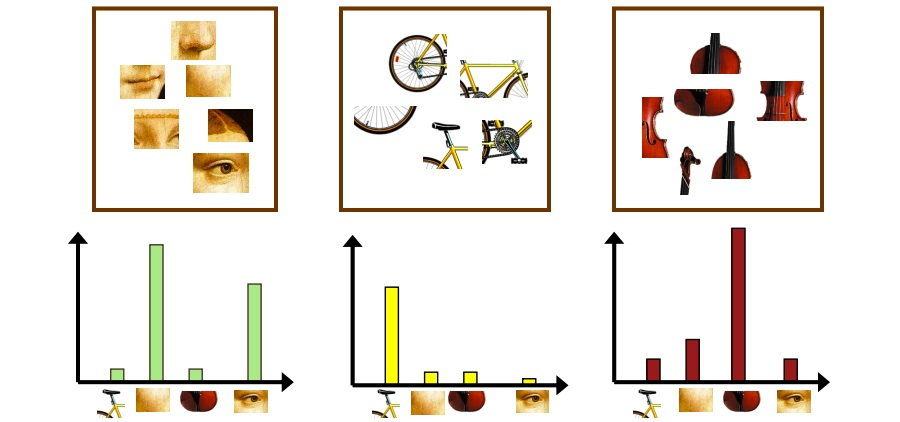
\includegraphics[scale=0.30]{wordhistogram.jpg}
\caption{Schematic representation of the bag-of-words system}
\label{wordhistogram}
\end{figure}

\subsubsection{Training the Classifier}
For this task we need to provide the Support Vector Machine with training instances as well as with the label of those instances. To do that we simply go through the training folders in our data, sample some instances (the ammount of which will be thoroughly explained in the Evaluation section) and alongside those instances we create a class label vector which contains the corresponding class of the instance.

Now having the obtained the training instances we are ready to train a multi-class SVM for image classification.

\section{Experiments and Evaluation}
In this section we will show the experiments we conducted alongside the parameters we used per experiment as well as the results we obtained for each of the experiment setups.

\begin{table}
\begin{tabular}{c|ccccc}
 & dense & keyPoints & RGB & rgb & opponent \\ 
\hline 
400 & • & • & • & • & • \\ 
800 & • & • & 75,5 & • & • \\ 
1600 & • & • & • & • & • \\ 
2000 & • & • & • & • & • \\ 
4000 & • & • & • & • & • \\ 
\end{tabular}
\label{Accuracy of the different models}
\end{table}

\section{Conclusion}

\bibliography{biblio.bib}{}
\bibliographystyle{plain}
\end{document}